\chapter{Algoritm Implementation}
Her tager vi de krav som vi har fundet i development og de krav som vi har bestemt i requirements og skal finde fx en platform som opfylder dem (se platform section). Vi skal også finde ud af hvordan man så kan omdanne vores matematiske / matlab algoritme til kode

\section{Platform (BlackFin)}
Her beskriver vi alle de ting som gør at vi har valgt BlackFin og de overvejelser der har været i forbindelse med det. Alt fra valget på baggrund af tilgængelig, interesse og andet over initializering og talkthrough til bufferstørrelser, MDA, implementeringskoden (den indbyggede og vores egen)

We have worked with several different platforms throughout the courses in our education. A valid choice for platform would be the PSoC 3(5) that we had already worked on. We had been told from other students taking this course that the PSoC was not ideal for sound processing and that the blackfin platform had built in features for this. We had no idea how to use the blackfin so it was a great opportunity to learn to use another platform. 
\subsection{PSoC}
\textbf{Speed:}\\
The PSoC 3 system has a single core running up to 67 MHz. It does not have fixed point arithmetic calculation so it might not be ideal for large DSP operations such as cross correlation. \\
\textbf{I/O:}\\
The PSoC has 28 GPIO pins. These can be configured any way you want. The range of the pins is 1.7 V to 5.5 V depending on supply voltage. \\
\textbf{ADC/DMA:}\\
PSoC has a 24-channel DMA which is programmable to access nearly every bus on the board. It has both delta-sigma and sar ADC with up to 20 bits resolution. Sample rate can be up to 192 kHz at 12 bit resolution. \\
\textbf{Memory:}\\
The PSoC has 64 KB of flash memory, 8 KB SRAM and 512-byte cache. This would be enough memory for small signals but would prove difficult if we were to use larger audio signals.\\
\subsection{Blackfin}
\textbf{Speed:}\\
The blackfin processor runs at 600MHz. For every clock it can do two operations (multiplication and/or addition). This effectively means that we can do 1200 million operations per second, if we use the processor 100\% of the time.\\
\textbf{I/O:}\\
The blackfin has an output range of 0 - 0.4 V low to 2.4 - 3.6 high. Input range is -0.3 to 3.6 V. Most of the blackfins I/O is controller by ports. All the phono plugs are connected to the port "Sport0". \\
\textbf{ADC \& Audiocodec:}\\
The blackfin has a built-in audiocodec consisting of 4 ADCs and 6 DACs with a resolution of 24 bits. It has a signal to noise ratio of 105dB\footnote{http://www.analog.com/en/audiovideo-products/audio-codecs/ad1836/products/product.html}. There is an example project in the VisualDSP++ environment explaining how to utilize this codec.\\
\textbf{Memory:}\\
Since we do not use much memory we use the L1 cache in the BF533. It is according to the datasheet 32Kbytes big. Since we work with the datatype "short", which is 16 bits, we have enough space for 16K samples.\\
\begin{figure}[hbpt]
\centering
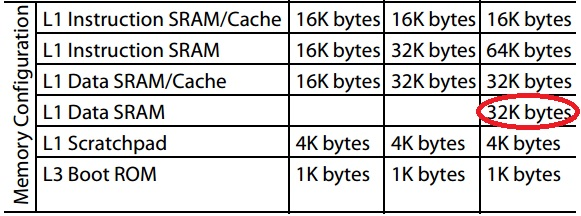
\includegraphics[width=0.5\textwidth]{billeder/memorytable}
\caption[Screen dump from datasheet]{Screen dump from datasheet\footnotemark}
\label{img:mem_table}
\end{figure}
\footnotetext{\url{http://www.analog.com/static/imported-files/data_sheets/ADSP-BF531_BF532_BF533.pdf}}
\subsection{DK8K}
We chose to ignore the DK8K platform as it does not have an Interactive Developer Environment(IDE). This would put a bigger workload on us but would not help us understand how to take advantage of Digital signal processing on embedded units.
\section{Our choice: the Blackfin}
\subsection{Output}
\textbf{UART}:\\
VisualDSP++ comes with an example project for UART. We tried running the example project but we had no luck. We could not get the example project to work. We searched the internet for other example projects but still, we could not get them to work. \\
\textbf{Sound}:\\
The original scope of our project was to have an audio source as our output, while using a sound to measure distance. This worked well since we already had the knowledge from the talkthrough on how to output sound.\\
We have a multitude of ways to create the sound we are playing. We could either create a sound in matlab and load it or we could create it directly on the blackfin. For testing purposes we chose the matlab solution. This would mean that once we have made the soundbits we wanted to use, we would have to convert them to a format known by the blackfin.
\subsection{Memory}
The blackfin has 2 types of memory: Internal and external. The internal SRAM consist of fast memory that is close to the processor.  As previously mentioned the L1 Data SRAM size is 32K Bytes. If we were to chose large arrays for our sound array we could enable the external SDRAM as well. This would provide us with a grand total of 132M bytes of memory. The SRAM is based on Harvard Architecture which makes it as fast as the processor. The SDRAM runs slower than the SRAM, so it would be ideal to confine the project to SRAM only. Enabling the SDRAM is done in VisualDSP++ by entering Project Options. The path would then be:
\begin{verbatim}
Project -> Link -> Processor (1) -> Memory Usage
\end{verbatim}

\subsection{DMA}
The is a controller circuit on embedded units that can initiate memory read or write cycles. Before the DMA controller can be used we have to initiate it. This is largely platform specific and the way we do it on the blackfin will be described in the algorith implementation chapter. The DMA controller on the blackfin can move data between L1 Cache, Flash or SDRAM and units connected to the DMA Access Bus. The Scope of our project means that we have to use Sport0 (which will be connected to the audio connectors) and internal memory from the L1. \\

\subsection{Resources}
Regarding resources on the blackfin we are looking to try to make our own implementation through the project and then compare with the built-in function. We are not trying to do it better but rather get the understanding of what is going on.
We also want to investigate the use of DMA on the blackfin so we do not waste resources on moving data only processing it.

\subsection{Buffer sizes}
We started by using 24000 size arrays. This means we had to use SDRAM. In an attempt to squeeze more performance out of our system we tried to limit ourselves to SRAM. The largest possible c style short array would be around 16000 elements. The next step was to try cross correlation with 2 16000 element signals. The cross correlation look strange and somehow some of the cross correlation array was assigned to "unassigned" memory space.\\
The next step in the choice of buffer size was to look at the arrays we made in matlab. We asked ourselves what the smallest possible array with chirp and noise we could play with 48kHz was. We tried playing a 1000 sample chirp and found that it didn't play properly. The next step was to double the size to 2000. This time the chirp played properly.\\
The last step was to think about the speed of sound. \fixme{johnnys story about bigger buffers and the speed of sound}

\subsection{Convert to BF}
The blackfin has a small "hack" when it comes to loading sound from memory:
\begin{lstlisting}[language=C]
short sound_buffer[length_of_signal] = { 
#include "signal_you_want_to_use.hex"
};
\end{lstlisting}
This means we have to convert our sound array to a hex format. The first thing we do when converting is reducing the amplitude of the signal to make sure it fits in a "c style short" datatype. Then we use a function "mydec2hex" which is an improved version of matlabs built-in function "dec2hex". After converting to hex-format we use the file descriptor to save the data into a hex file. The hex file is put in the project folder in VisualDSP++ and the codehack is put where you initialize your variables.



\subsection{IDE: VisualDSP++}
\subsubsection{Plot}
VisualDSP++ has a built-in function to plot data from the memory of the blackfin. This feature can be used when the blackfin has been flashed and then subsequently halted. To access this feature go into:
\begin{verbatim}
View -> Debug Windows -> Plot -> New
\end{verbatim}
Set name, length and type of the data you want to plot and press \"Add\". This way you can have multiple plots on the same graph. It is also possible to have multiple plots and to save the setting of your plot. An example of plot can be seen on figure~\ref{fig:visualdspplot}.
\begin{figure}[hbpt]
\centering
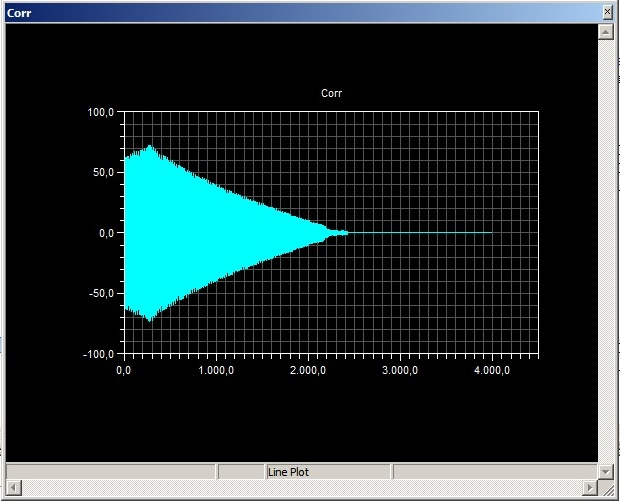
\includegraphics[scale=0.5]{billeder/visualdspplot}
\caption{Plot in VisualDSP++}
\label{fig:visualdspplot}
\end{figure}
\subsubsection{Memory dump}
A useful feature in VisualDSP++ is Memory dump. We can save the contents of arrays and variables directly onto the computer running VisualDSP++ in ".dat" format. To access this feature go into:
\begin{verbatim}
Memory -> Dump
\end{verbatim}
Set filename, type, size and variable/array name. Matlab can import these files directly.

\section{Fixed-/FloatingPoint}
\subsection{Floating Point}
Floating point is a way of give approximation of a real value. Usually when working with floating point we have a fixed number of significant digits. A way of presenting a floating point number is "1.2345". Floating point types in c are double and float. The main advantage of floating point is high precision. This comes at a cost of performance and component price.\\
\subsection{Fixed Point}
Fixed point arithmetic is a way to represent a number that has a fixed number of digits before and after the the decimal "." point. Fixed point arithmetic is especially useful for representing fract data types in base 2 or base 10. A way to represent "1.23" in fixed point is "1230". A scaling factor was used. Scaling factors are usually base 2 or base 10. The main advantage of fixed point is performance. This comes at a price of precision. Some embedded microprocessors can not process floating point as it requires a floating point unit(FPU).\\
\subsection{Choice}
The blackfins built in fixed point arithmetic system makes it ideal to operate in fixed point. Our systems real time demand means we have to have great performance which leads to the choice of using fixed point arithmetic throughout the our system. A performance example would be to multiplication of variables. Table~\ref{tab:performance} shows some clock-cycle readings from multiplication. The table clearly shows that the best performance is found using assembly and short data types, but we chose to write everything in c using short data types because that is what we were most familiar with.
\begin{table}[hbtp]
	\centering
    \begin{tabular}{| p{4.5cm} | p{2.5cm} |}
    \hline
    Format                   & Clock cycles \\ \hline
    C style integer, 32 bit  & around 3000  \\ \hline
    Assembly integer, 32 bit & around 500   \\ \hline
    Float                    & around 16000 \\ \hline
    Assembly short, 16 bit   & around 70    \\ \hline
    \end{tabular}
    \caption{example of multiplication performance table}
    \label{tab:performance}
\end{table}

\section{Blackfin Setup}
\subsection{DMA}
The DMA is setup using SPI on the blackfin. We have used code from the example project "Audio Talk-Through" Which initiates the dma channels 1, 2 and 5 for input, output and moving data to the built in audio codec. The DMA has the following init parts:
\begin{lstlisting}[language=C]
*pDMA1_PERIPHERAL_MAP // What to map the DMA to.
*pDMA1_CONFIG // which configuration your want.
*pDMA1_START_ADDR // Start address of the buffer.
*pDMA1_X_COUNT // Number of transfers
*pDMA1_X_MODIFY // Number of bytes between each transfer
\end{lstlisting}
In our setup we are using 32 bytes so the DMA in- and output are set to 32 bytes, 8 bursts of 4 bytes at a time. We map the in and output dma channels to Sport0 Rx and Tx. Sport0 is connected to our physical ports described below. The last thing we have to do is enable the DMA channels and that is done with the \begin{quote}
"DMAEN" flag in the "pDMA1\_CONFIG".
\end{quote}
\subsection{Sport0}
The Sport0 is set up using the table \ref{table:Sport0}
\begin{table}[htbp]
    \begin{tabular}{| p{1.5cm} | l | p{4.5cm} | p{4.5cm} |}
    \hline
    C++ def      & Comment                   & Clear bit to 0                                   & Set bit to 1                             \\ \hline
    TFSR RFSR   & Frame sync required 		 & Does not require frame sync for every word & Requires frame  					sync for every word \\ \hline
    ITFS IRFS   & Internal frame  					sync & Use external  					frame sync                    & Use internal  					frame sync            \\ \hline
    ITCLK IRCLK & Internal clock            & Use external  					clock                         & Use internal  					clock                 \\ \hline
    TSPEN RSPEN & Enable                    & Disable transmit  					or receive                & Enable transmit  					or receive         \\ \hline
    \end{tabular}
    \caption{Sport0 Initialization}
    \label{table:Sport0}
\end{table}
Our Sport0 is set up the same way as the "talkthrough" project with: "External CLK, External Frame sync, MSB first". MSB first is instantiated by writing SLEN$\_$32 to the second register. Lastly we enable it by writing "TSPEN" and "RSPEN" to the registers pSPORT0 TCR1 and RCR1.
\subsection{Interrupts}
Interrups are set up using the 4 registers SIC$\_$IAR0 to 2 and SIC$\_$IMASK. We want to use DMA1 (Sport0 RX) Interrupt so we set the second word of the SIC$\_$IAR1 to 2. We also have to register ISR handlers to Sport0 and then enable interrupt. The interrupt code will then be:
\begin{lstlisting}[language=C]
*pSIC_IAR0 = 0xffffffff;
*pSIC_IAR1 = 0xffffff2f; // DMA1 (Sport0 RX)
*pSIC_IAR2 = 0xffffffff;

register_handler(ik_ivg9, Sport0_RX_ISR); //Handler

*pSIC_IMASK = 0x00000200; // enable interrupt
\end{lstlisting}

\section{System overview/architecture}
hest

\section{Code functions}